\documentclass[11pt]{article}

\usepackage[margin=1in]{geometry}
\usepackage{booktabs}
\usepackage{graphicx}
\usepackage{parskip}
\usepackage{enumitem}
\usepackage{hyperref}

\title{\textbf{Dataset Profile EDA Report}\\[4pt]
Raw Data Profiling Before VPR Experiments}
\author{Rhoda Ojetola \and Peter Adeyemo \and Samuel Olusola}
\date{April 24, 2026}

\begin{document}
\maketitle

\section*{Purpose}
This report focuses on \textbf{raw dataset profiling before any descriptor experiments}. The goal is to understand what the datasets already tell us on their own:
\begin{itemize}[leftmargin=*]
  \item how large they are,
  \item whether the splits are balanced,
  \item whether day and night images follow similar distributions,
  \item whether the campus query set is dominated by hard no-match cases, and
  \item whether the campus walk is evenly covered across places.
\end{itemize}

The profiling code is in \texttt{analysis/dataset\_profile\_eda.py}, and the generated plots are saved under \texttt{output\_images/eda/data\_profiling/}.

\section*{Question 1: Are the datasets balanced at the split level?}
\textbf{Answer:} GardensPoint is balanced, but campus is smaller and less balanced.

\begin{center}
\begin{tabular}{lcc}
\toprule
\textbf{Dataset} & \textbf{Database / Day} & \textbf{Query / Night} \\
\midrule
GardensPoint & 200 & 200 \\
Campus strict & 50 & 64 \\
\bottomrule
\end{tabular}
\end{center}

\textbf{Interpretation.}
\begin{itemize}[leftmargin=*]
  \item GardensPoint behaves like a clean benchmark split.
  \item The campus dataset is much smaller, so each difficult example has a larger effect on the final metrics.
  \item This matters experimentally because variance will be lower on GardensPoint and much higher on campus. A small gain or drop on campus should therefore be read more cautiously, especially when only a few hard queries can move the metric noticeably.
\end{itemize}

\section*{Question 2: Are image sizes and aspect ratios consistent?}
\textbf{Answer:} GardensPoint day and night images do \textbf{not} share the same resolution, while the campus data is size-consistent.

\begin{figure}[h!]
\centering
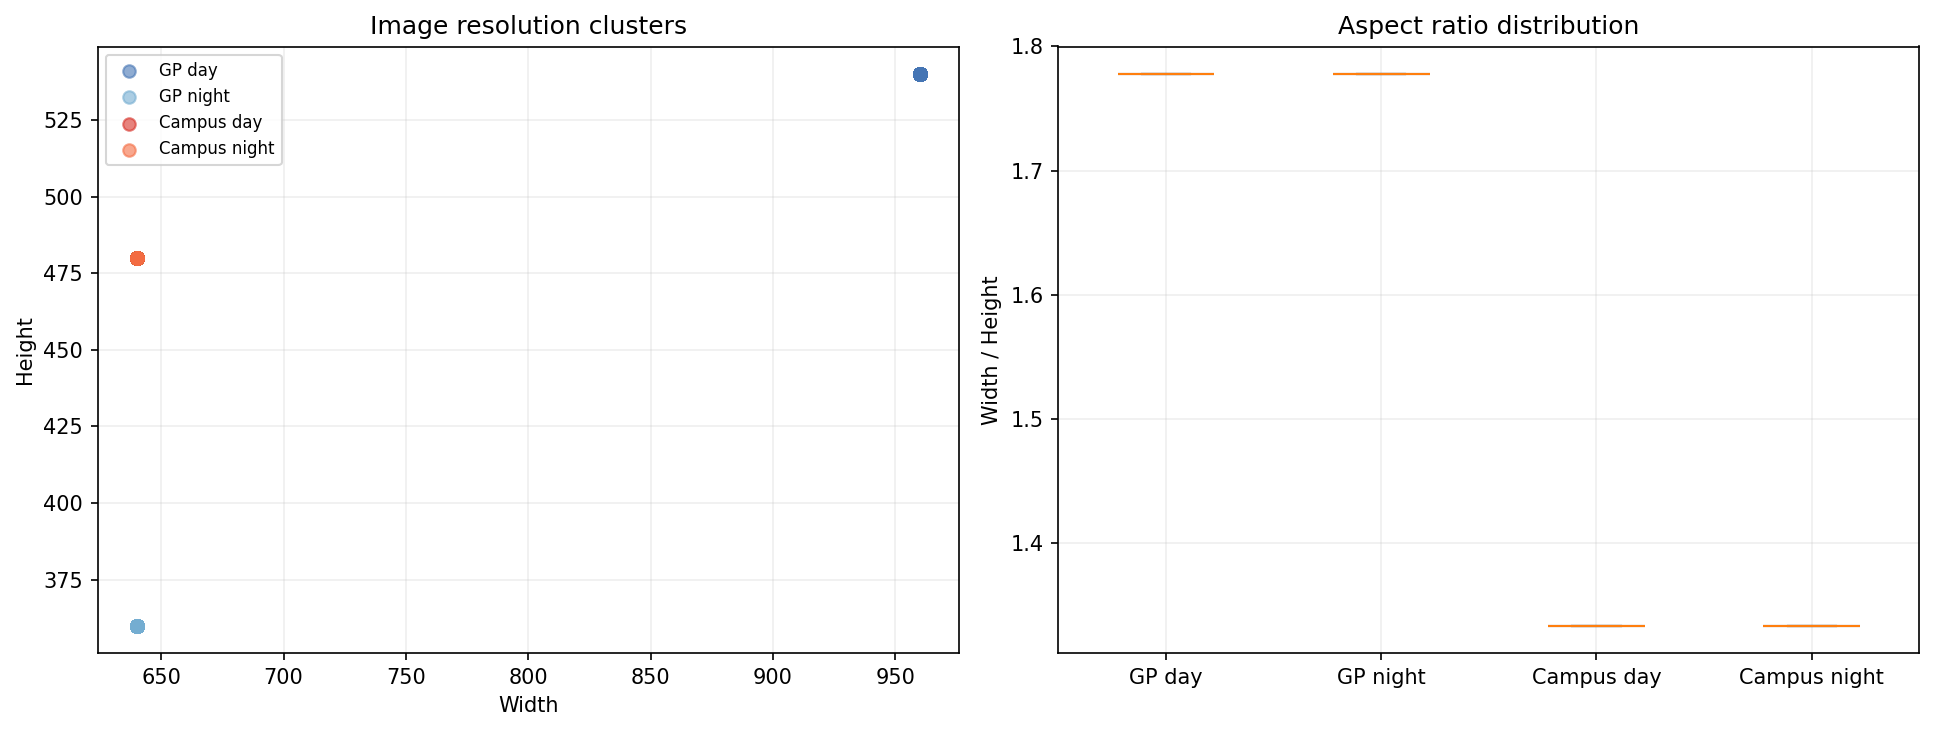
\includegraphics[width=0.88\textwidth]{../../output_images/eda/data_profiling/image_size_distributions.png}
\caption{Resolution and aspect-ratio profiling before any descriptor extraction.}
\end{figure}

\begin{itemize}[leftmargin=*]
  \item GardensPoint day images average \textbf{960x540}.
  \item GardensPoint night images average \textbf{640x360}.
  \item Campus day and night images both average \textbf{640x480}.
\end{itemize}

\textbf{Interpretation.} This means the benchmark already contains a raw size mismatch between day and night, while campus difficulty comes from content and illumination rather than image size. In practice, resizing inside the descriptor pipeline may hide this difference partially, but the EDA still tells us that GardensPoint and campus are stressing the model in different ways before any features are extracted.

\section*{Question 3: How different are the raw day and night image distributions?}
\textbf{Answer:} The two datasets show \textbf{different kinds of night-time shift}.

\begin{figure}[h!]
\centering
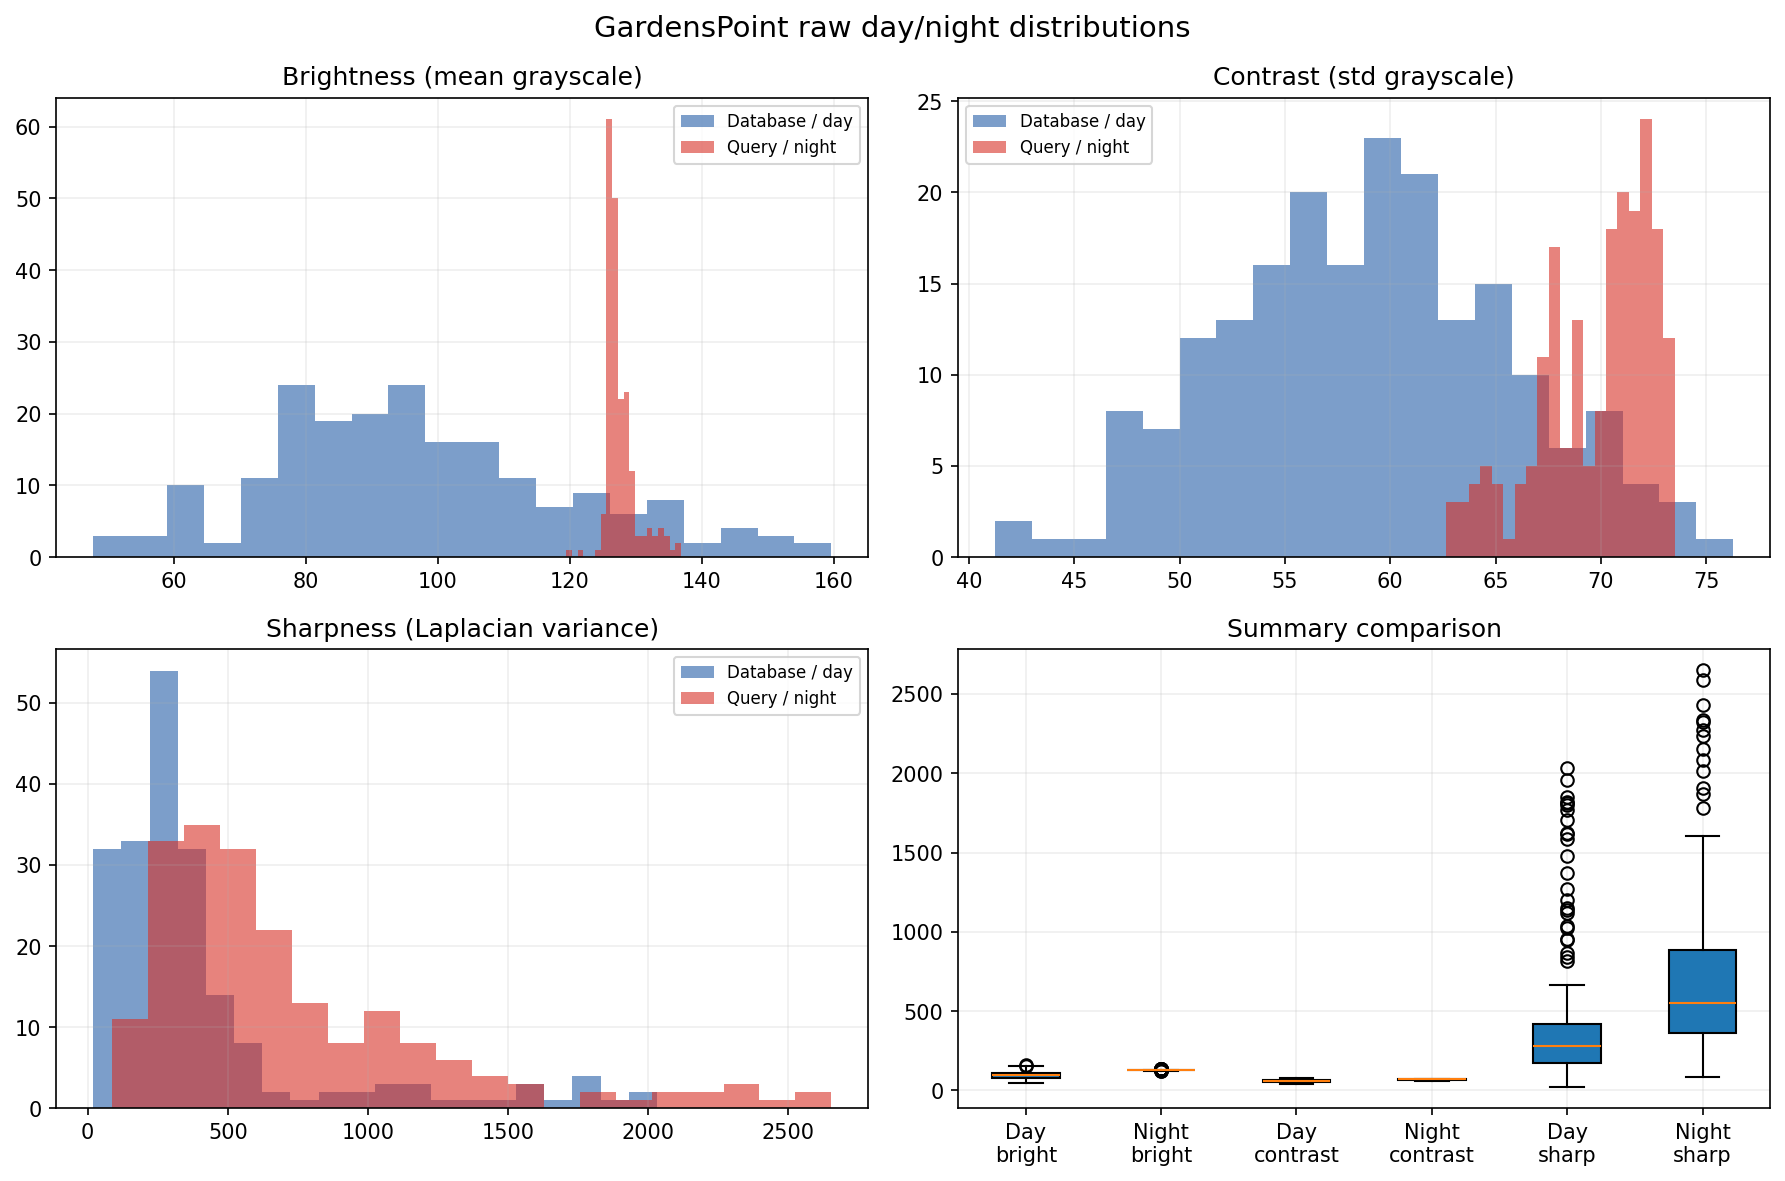
\includegraphics[width=0.86\textwidth]{../../output_images/eda/data_profiling/gardenspoint_raw_distributions.png}
\caption{Raw day versus night distributions on GardensPoint.}
\end{figure}

\begin{figure}[h!]
\centering
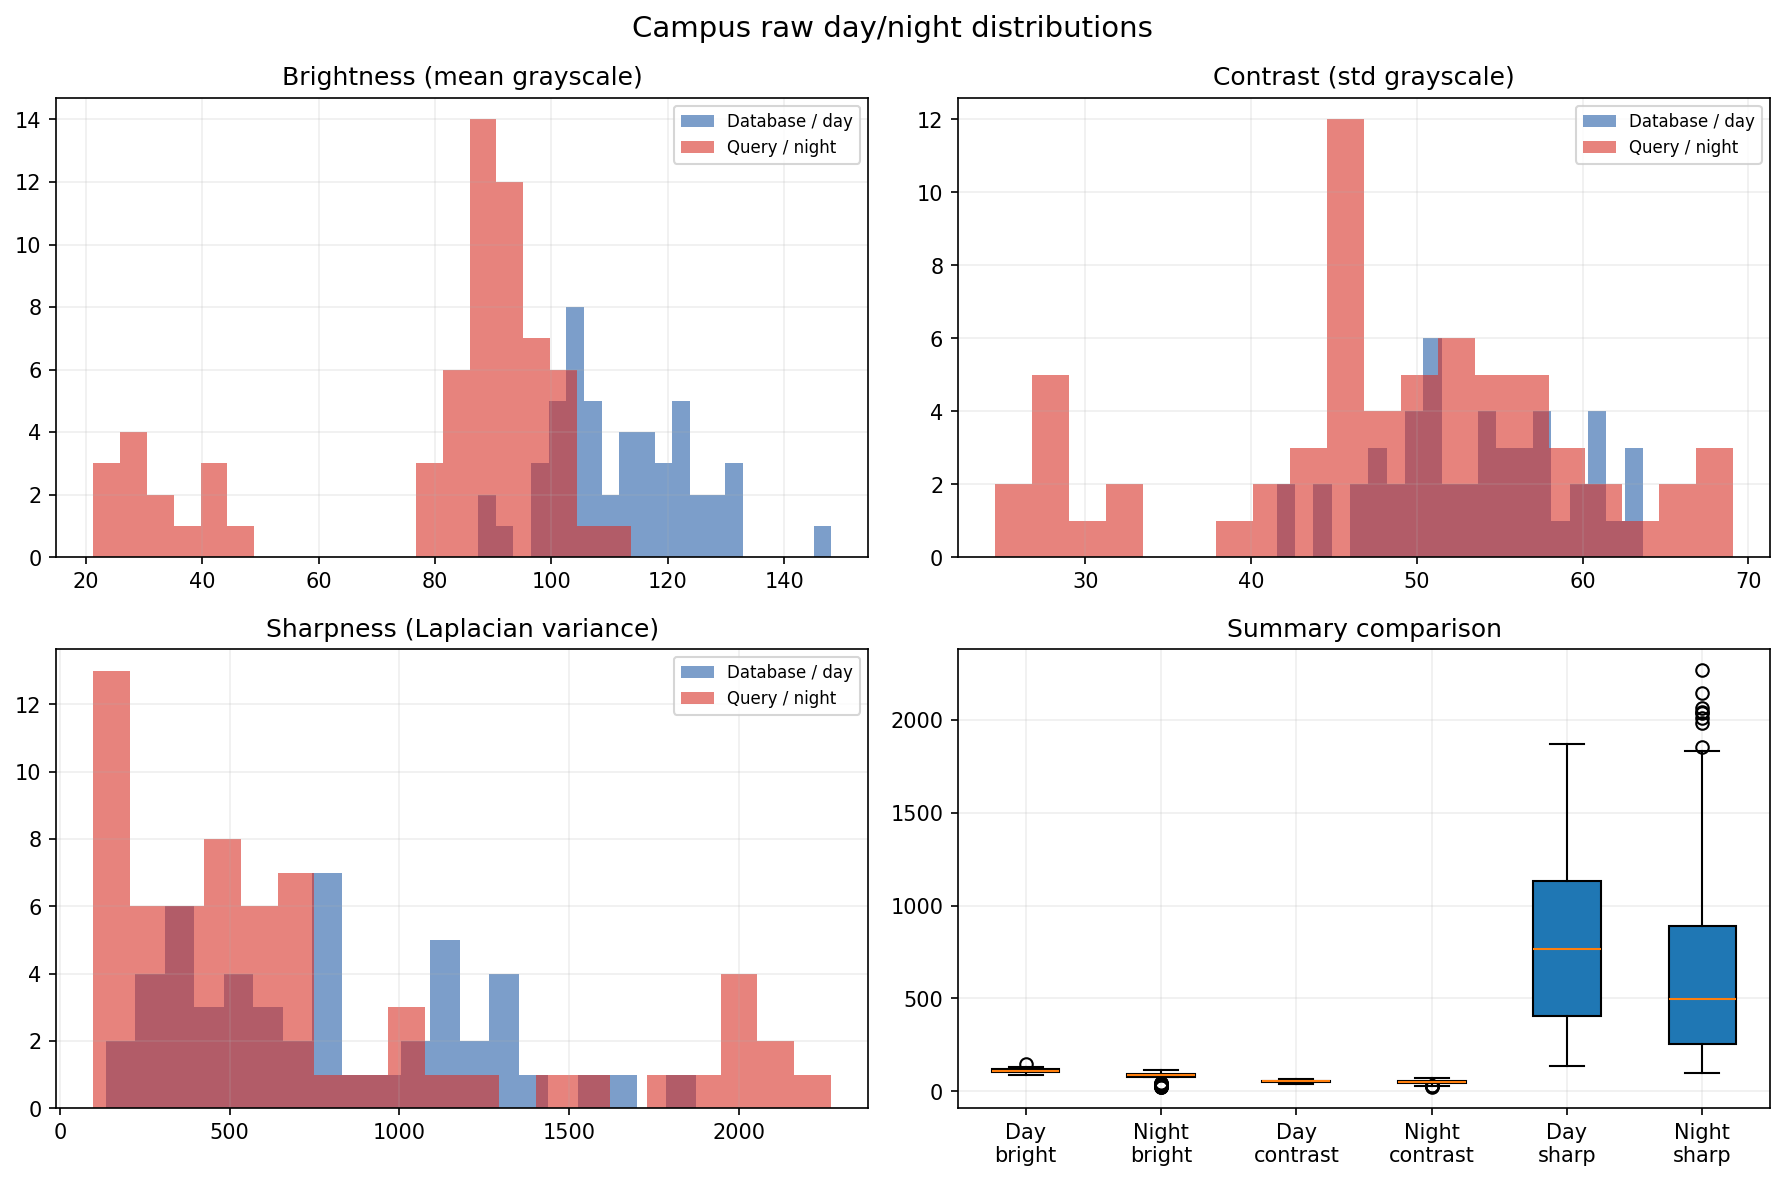
\includegraphics[width=0.86\textwidth]{../../output_images/eda/data_profiling/campus_raw_distributions.png}
\caption{Raw day versus night distributions on the campus dataset.}
\end{figure}

\begin{center}
\begin{tabular}{lccc}
\toprule
\textbf{Split} & \textbf{Brightness Mean} & \textbf{Contrast Mean} & \textbf{Sharpness Mean} \\
\midrule
GardensPoint day & 97.1 & 58.9 & 405.8 \\
GardensPoint night & 127.6 & 69.8 & 718.3 \\
Campus day & 112.0 & 53.5 & 784.2 \\
Campus night & 79.1 & 48.4 & 719.7 \\
\bottomrule
\end{tabular}
\end{center}

\textbf{Interpretation.}
\begin{itemize}[leftmargin=*]
  \item On GardensPoint, night images are \textbf{brighter}, higher-contrast, and sharper than day images.
  \item On campus, night images are \textbf{darker} and slightly lower in contrast.
  \item Visually, the GardensPoint night frames appear \textbf{exposure-compensated or over-brightened}, rather than simply representing a naturally dark night condition. The EDA is consistent with that impression.
  \item So GardensPoint and campus do not represent the same visual night condition. This is one reason why a descriptor can look strong on GardensPoint and still struggle to transfer fully to campus.
  \item Conceptually, this is why raw-distribution EDA matters: if the benchmark night split is artificially brightened, then benchmark success may reflect robustness to viewpoint and route alignment more than robustness to truly dark night imagery.
\end{itemize}

\section*{Question 4: How challenging is the strict campus query composition before any model is used?}
\textbf{Answer:} The campus strict query set is hard even before descriptor extraction because many queries are not simple one-to-one matches.

\begin{figure}[h!]
\centering
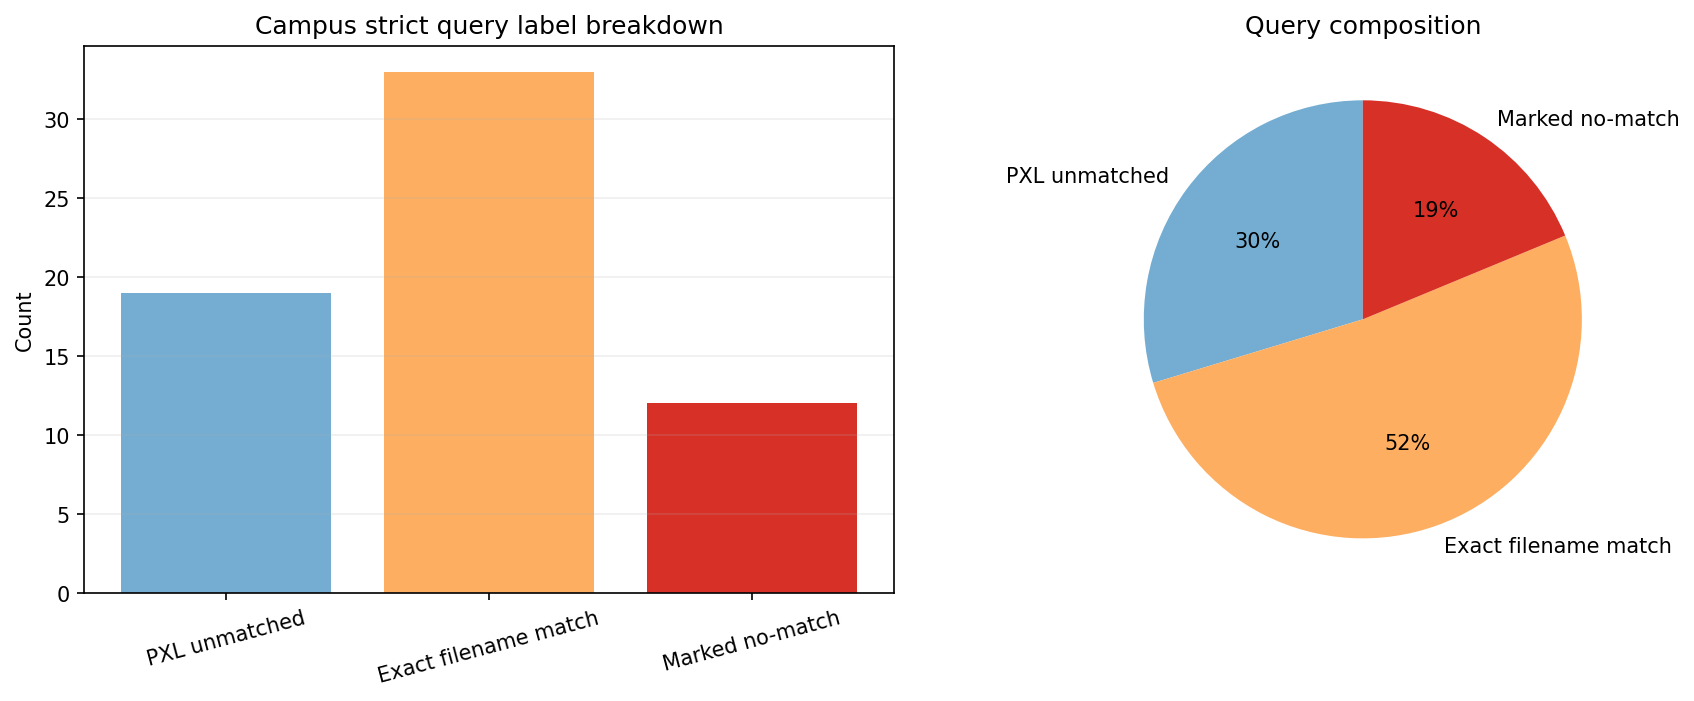
\includegraphics[width=0.82\textwidth]{../../output_images/eda/data_profiling/campus_strict_query_composition.png}
\caption{Strict campus query composition before experimentation.}
\end{figure}

The strict campus query split contains:
\begin{itemize}[leftmargin=*]
  \item \textbf{33} exact filename matches,
  \item \textbf{12} marked no-match queries, and
  \item \textbf{19} \texttt{PXL\_*} phone images with no strict day counterpart.
\end{itemize}

\textbf{Interpretation.} Nearly half the strict campus query set is effectively a hard rejection or non-one-to-one retrieval problem. This means low precision-style metrics on campus are not only a descriptor issue; they are also a dataset-structure issue. These \texttt{PXL\_*} images are still part of the strict dataset and are intentionally kept as hard no-match queries. So before running any model, the EDA already warns us that thresholded matching will be much harder than top-\(k\) retrieval.

\section*{Question 5: Is place coverage balanced across the campus walk?}
\textbf{Answer:} No. The place-level annotations show clear imbalance.

\begin{figure}[h!]
\centering
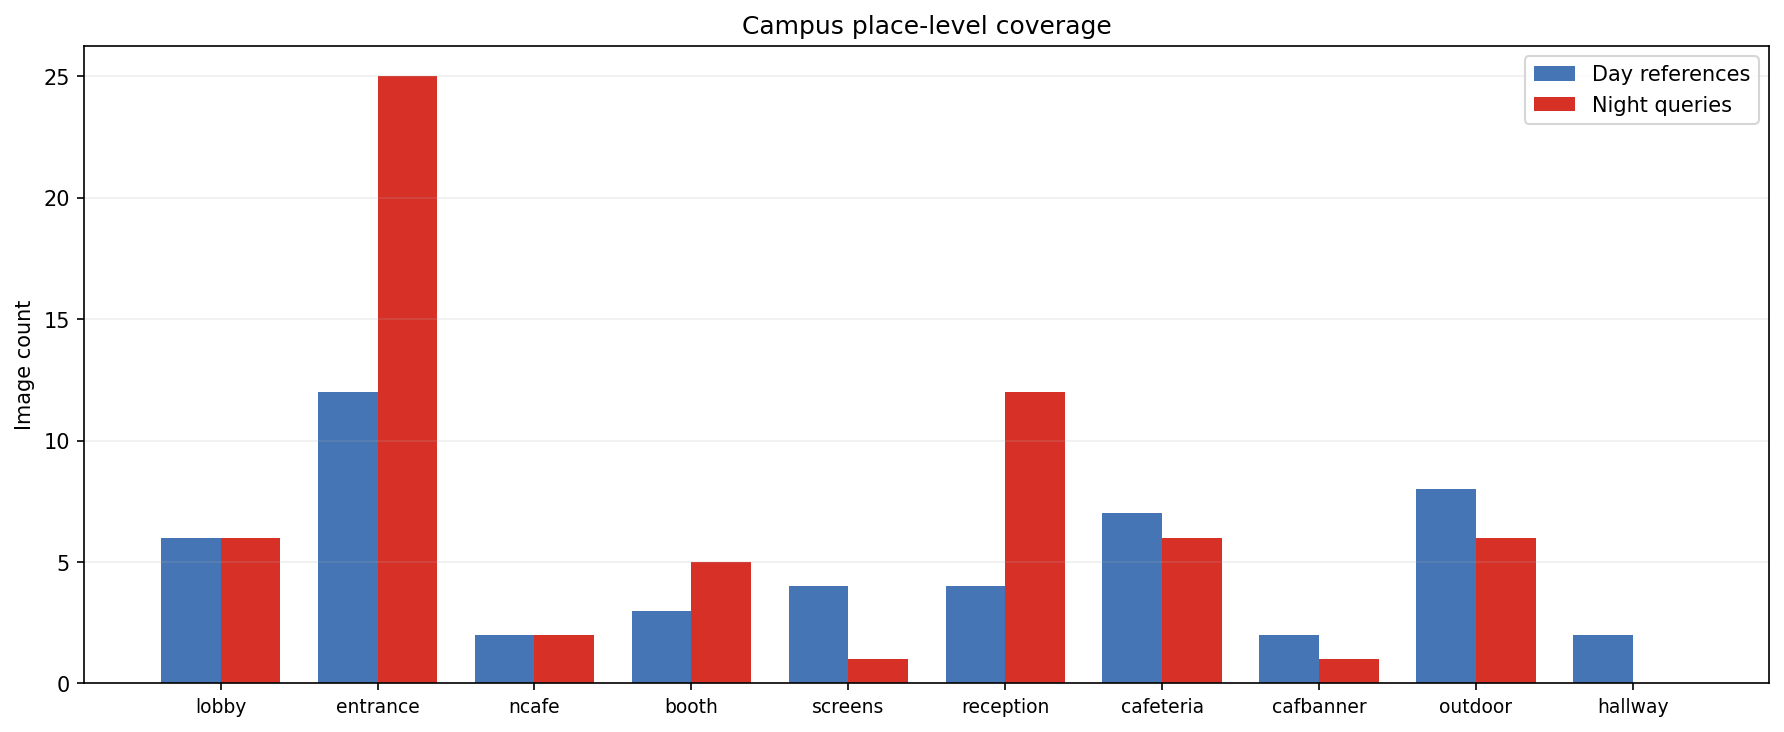
\includegraphics[width=0.95\textwidth]{../../output_images/eda/data_profiling/campus_place_coverage.png}
\caption{Place coverage across the campus walk.}
\end{figure}

\textbf{Main observations.}
\begin{itemize}[leftmargin=*]
  \item There are \textbf{10} unique place IDs.
  \item The largest night bucket is \textbf{\texttt{entrance}} with \textbf{25} images.
  \item Some locations have very limited support, and \texttt{hallway} has no night counterpart in the rematched place-level flow.
\end{itemize}

\textbf{Interpretation.} The campus walk is not uniformly sampled, so some regions will dominate retrieval behavior more than others. In practice, descriptors will see many more examples of \texttt{entrance} than of smaller places such as \texttt{ncafe} or \texttt{cafbanner}. That means a model can appear strong simply because the most common places are easier to retrieve, while underrepresented places may stay fragile. This is why the place-coverage EDA matters before experimentation: it tells us that raw dataset frequency can bias which scenes dominate the final metrics.

\section*{Question 6: What do representative samples look like?}
\textbf{Answer:} The montages confirm the statistical findings visually.

\begin{figure}[h!]
\centering
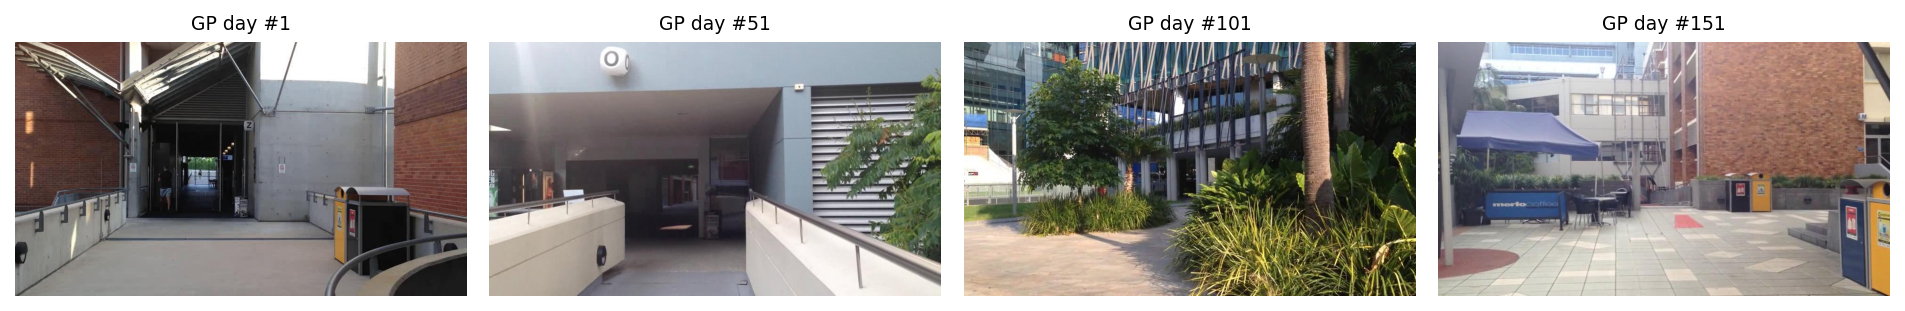
\includegraphics[width=0.9\textwidth]{../../output_images/eda/data_profiling/gardenspoint_day_montage.png}\\[0.4em]
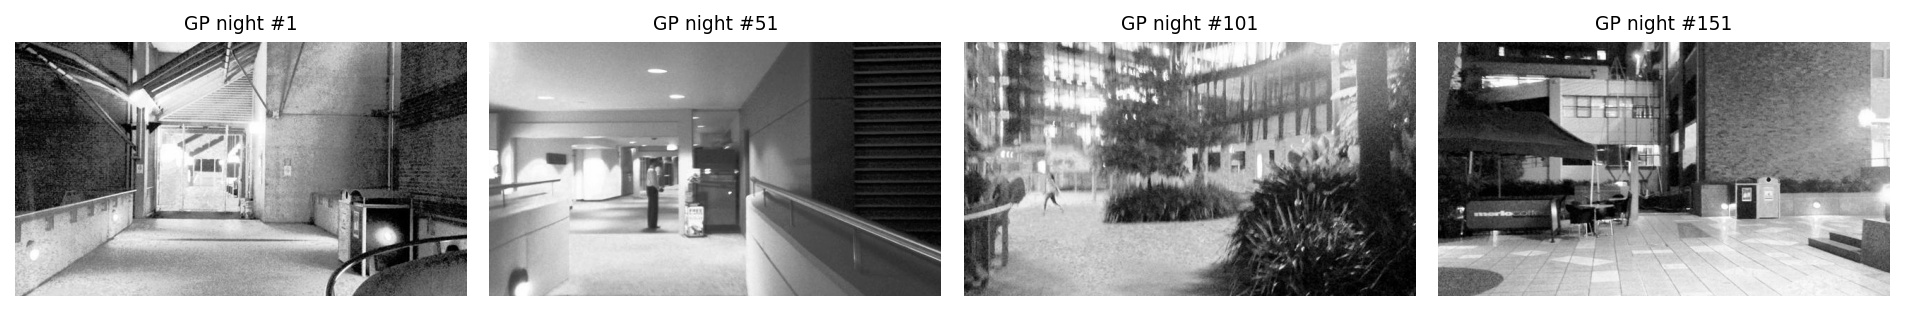
\includegraphics[width=0.9\textwidth]{../../output_images/eda/data_profiling/gardenspoint_night_montage.png}
\caption{Representative GardensPoint day and night samples.}
\end{figure}

\begin{figure}[h!]
\centering
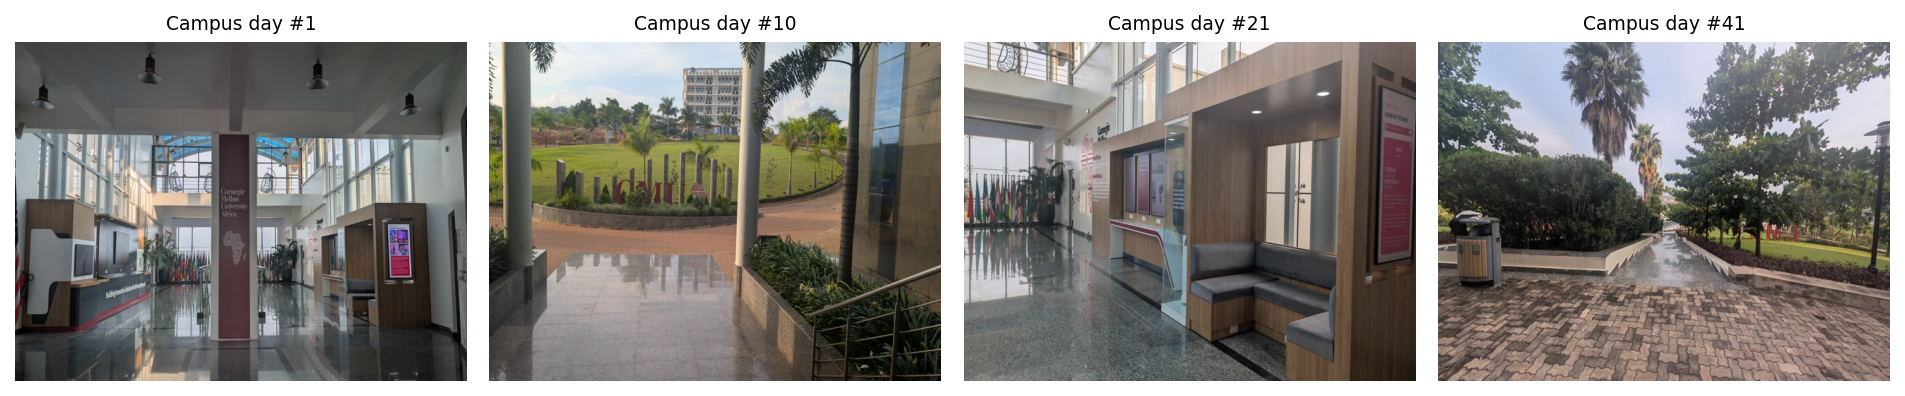
\includegraphics[width=0.9\textwidth]{../../output_images/eda/data_profiling/campus_day_montage.png}\\[0.4em]
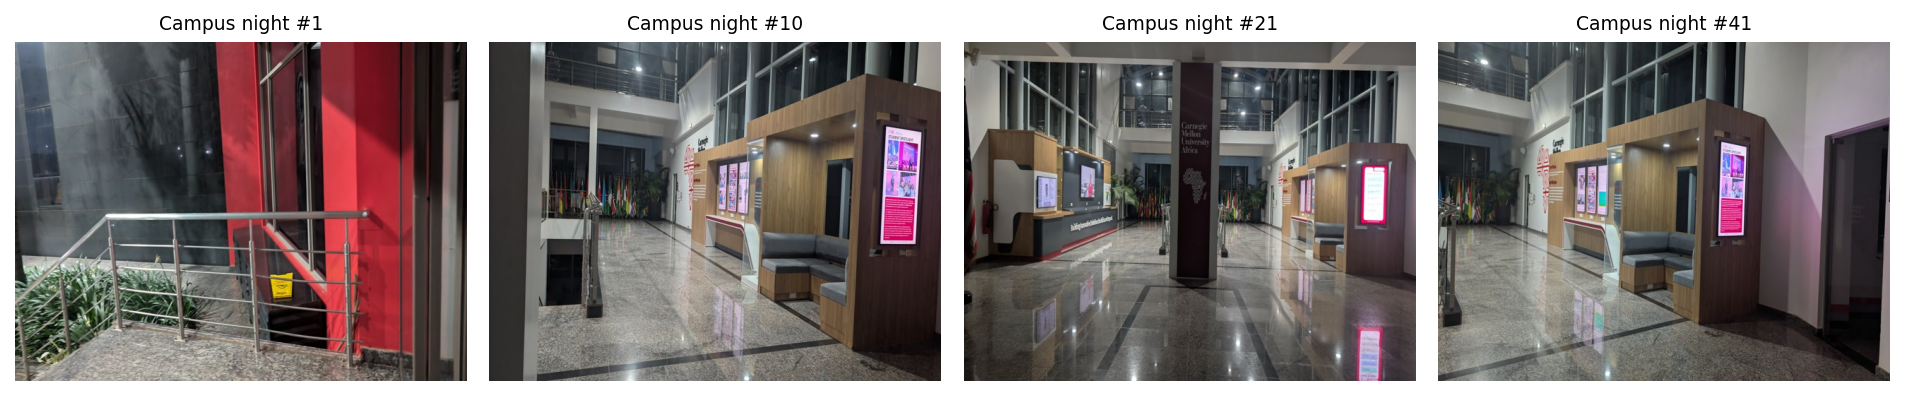
\includegraphics[width=0.9\textwidth]{../../output_images/eda/data_profiling/campus_night_montage.png}
\caption{Representative campus day and night samples.}
\end{figure}

\textbf{Interpretation.}
\begin{itemize}[leftmargin=*]
  \item GardensPoint shows cleaner route progression and visually consistent nighttime lighting, but the night frames also look exposure-lifted, which helps explain why their average brightness is unexpectedly higher than the day split.
  \item Campus shows stronger viewpoint variation, more uneven lighting, and more heterogeneous scenes, so it is a better stress test for transfer but a noisier benchmark for clean descriptor comparison.
\end{itemize}

\section*{Conclusion}
This profile EDA shows that the raw data itself already explains part of our later experimental behavior:
\begin{itemize}[leftmargin=*]
  \item GardensPoint is a useful controlled benchmark, but its night distribution is not identical to campus.
  \item The campus strict split is difficult before any model is even chosen because of its no-match composition.
  \item The campus walk is also unevenly sampled across places.
\end{itemize}

So the raw data supports our experimental design: use GardensPoint as the controlled benchmark, use campus as the harder transfer test, and interpret campus results with an awareness of label composition and place imbalance. More importantly, this EDA gives us a checklist for reading later experiments correctly: benchmark gains do not automatically imply campus robustness, precision-style failures may come from query composition rather than descriptor weakness alone, and strong scores on common places do not guarantee balanced performance across the whole route.

\end{document}
